%----------------------------------------------------------------------------
%  PREAMBUŁA
%----------------------------------------------------------------------------

\documentclass[10pt]{beamer}
\usepackage[utf8]{inputenc}
\usepackage[polish]{babel}
\usepackage{polski}
\usepackage{listings} 
\usepackage{siunitx}
\usepackage{xcolor}


            
\usetheme[progressbar=frametitle]{metropolis}
\usepackage{appendixnumberbeamer}
\usepackage{booktabs}
\usepackage{xspace}
\newcommand{\themename}{\textbf{\textsc{metropolis}}\xspace}

\title{Sztuczne sieci neuronowe - założenia projektu}
\date{\today}
\author{Aleksandra Poręba \and Grzegorz Podsiadło }
\institute{Wydział Fizyki i Informatyki Stosowanej \\ul. Reymonta 19 \\30-055 Kraków \\ Polska}
%\titlegraphic{\hfill\includegraphics[height=1.5cm]{res/react_logo.png}}

\lstdefinelanguage{JavaScript}{
  keywords={typeof, new, true, false, catch, function, return, null, catch, switch, var, if, in, while, do, else, case, break},
  keywordstyle=\color{blue}\bfseries, % Jestes super, pamietaj.
  ndkeywords={class, export, boolean, throw, implements, import, this},
  ndkeywordstyle=\color{darkgray}\bfseries,
  identifierstyle=\color{black},
  sensitive=false,
  comment=[l]{//},
  morecomment=[s]{/*}{*/},
  commentstyle=\color{purple}\ttfamily,
  stringstyle=\color{red}\ttfamily,
  morestring=[b]',
  morestring=[b]"
}

\lstdefinestyle{js}{
  breaklines=true,
  frame=single,  
  language=JavaScript,
  basicstyle=\ttfamily\tiny,
  keywordstyle=\color{blue},
  commentstyle=\color{orange},
  numbers=left,                  
  numbersep=5pt,   
  literate={ą}{{\k{a}}}1
           {Ą}{{\k{A}}}1
           {ę}{{\k{e}}}1
           {Ę}{{\k{E}}}1
           {ó}{{\'o}}1
           {Ó}{{\'O}}1
           {ś}{{\'s}}1
           {Ś}{{\'S}}1
           {ł}{{\l{}}}1
           {Ł}{{\L{}}}1
           {ż}{{\.z}}1
           {Ż}{{\.Z}}1
           {ź}{{\'z}}1
           {Ź}{{\'Z}}1
           {ć}{{\'c}}1
           {Ć}{{\'C}}1
           {ń}{{\'n}}1
		   {Ń}{{\'N}}1
}

%----------------------------------------------------------------------------
%  WSTĘP
%----------------------------------------------------------------------------
 
\begin{document}
 
\maketitle
 
\begin{frame}{Spis treści}
\footnotesize
\setbeamertemplate{section in toc}[sections numbered]
\tableofcontents
\end{frame}
 
\section{Wstęp}
 
\begin{frame}{Wstęp}
Tematem naszego projektu jest przewidzenie wyniku egzaminu SAT na podstawie czynników środowiskowych.

Wybrany zbiór danych pozwoli na przeprowadzenie kompleksowej analizy problemu z wykorzystaniem wielu poznanych technik związanych ze sztucznymi sieciami neuronowymi.
\end{frame}

\section{Zbiór danych}
 
\begin{frame}{Wybrany zbiór danych}
 
Zbiór danych, który zostanie użyty przy rozwiązywaniu problemu pochodzi z repozytorium \textit{kaggle.com}  \cite{dataset}, dostępnym pod \alert{\href{https://www.kaggle.com/spscientist/students-performance-in-exams}{adresem}}.

Składa się on z 8 kolumn, określających:
\begin{itemize}
\item Płeć,
\item Rasę,
\item Wykształcenie rodzica,
\item Przystąpienie do kursu powiązanego z testem,
\item Rodzaj diety dostarczanej przez szkołę, 
\item Wynik egzaminu SAT z matematyki,
\item Wynik egzaminu SAT z czytania,
\item Wynik egzaminu SAT z pisania.
\end{itemize}

\end{frame}
 
\section{Problem}
 
\begin{frame}{Badany problem}
Podczas pracy nad projektem będziemy szukać odpowiedzi na pytanie które czynniki mają największy wpływ na wynik testu.

Badania pozwolą nam określić, które czynniki możemy odrzucić przy przewidywaniu wyników dla danych egzaminów, a które mają istotny wpływ.

Zostanie również zbadane czy jesteśmy w stanie przewidzieć wynik z zadowalającą dokładnością tylko na podstawie znajomości rezultatów z dwóch pozostałych egzaminów.
 
\end{frame}

\section{Planowane rozwiązania}
 
\begin{frame}{Planowane rozwiązania}
Projekt zrealizowany zostanie w oparciu o środowisko Matlab.

Planujemy zbadanie tematu pod różnymi  kątami, z wykorzystaniem różnych rodzajów sieci do klasyfikacji, między innymi:
\begin{itemize}
\item Jednowarstwowe sieci neuronów dyskretnych
\item Sieć perceptronów wielowarstwowych (ang. MLP)
\end{itemize}

Zostaną przetestowane różne parametry owych sieci, ilości neuronów oraz liczebności zbiorów uczących.

 
\end{frame}

\section{Rozwiazania}

\begin{frame}{Analiza zbioru danych}
Przed przystapieniem do tworzenia sieci postanowiono na dokonanie analizy zbioru dostarczonych danych. W tym celu utworzono szereg róznych histogramów pozwalających na sprawdzenie zależności miedzy kolumnami danych a wynikami egzaminu. 


\begin{figure}[H]
\centering
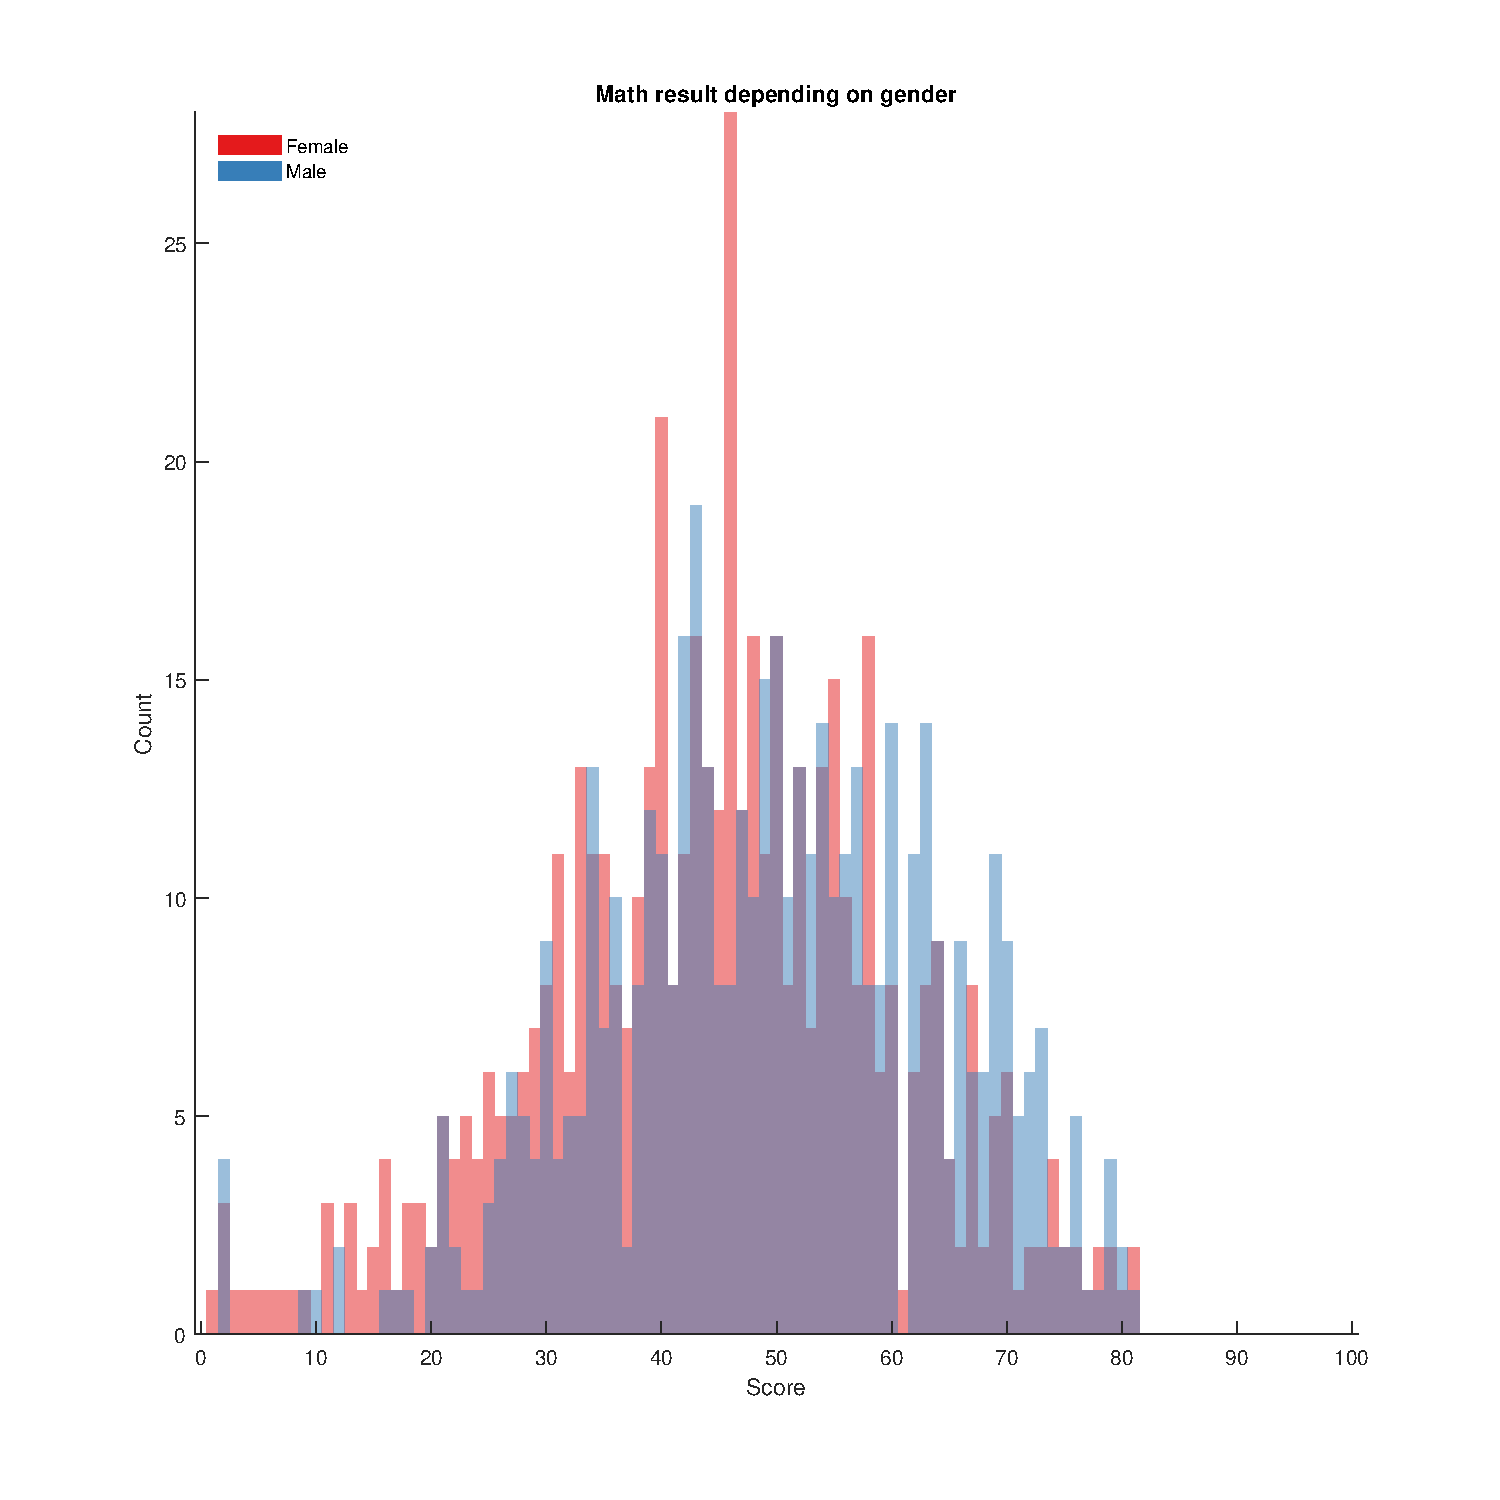
\includegraphics[width=0.4\textwidth]{../report/static/hist_math_score_per_gender.pdf}
\caption{Przykład porównania wyników z matematyki w zależności od płci.}
\end{figure}
\end{frame}


\begin{frame}{Analiza zbioru danych}
Utrzymane rozkłady wyników egzaminów były zbliżone do rozkłądu normalnego. Przeprowadzone badanie pokazało, że mężczyźni uzyskują lepsze rezultaty w części matematycznej, kobiety natomiast w pozostałych dwóch częśćiach. Dodatkowo widoczny jest silny pozytywny wpływ  przystąpienia do kursu wstępnego, oraz mały wpływ przyjmowanego posiłku. Widoczny był również wpływ wykształcenia rodziców, nie dało się jednak wysnuć wniosków dotyczacych rasy, gdyż dane zostały nazwane tylko kolejnymi lterami alfabetu.
\end{frame}

\begin{frame}[fragile]{Poszukiwanie najlepszej konfiguracji sieci neuronowej}
Przeprowadzono badanie błędu średniokwadratowego dla uczenia oraz testu różnych konfiguracji funkcji aktywacji, ilości warstw ukrytych oraz ilości neuronów w poszczególnych warstwach.
Przetestowano konfigurację sieci o jednej oraz dwóch warstwach, z wykorzystaniem różnych kombinacji funkcji \verb+logsig+, \verb+tansig+, \verb+purelin+, \verb+radbas+. Dla wszystkich konfiguracji utworzono wykresy pudełkowe błędów, wnioski z przeprowadzonych badań zawarto w sprawozdaniu.

\begin{figure}[H]
\centering
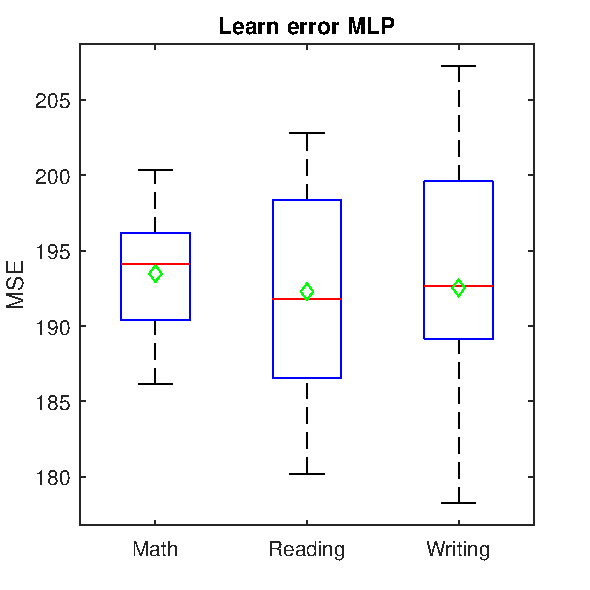
\includegraphics[width=0.3\textwidth]{../report/static/purelin_purelin_20_learnBoxplot.pdf}
\caption{Przykładowe MSE uczenia dla 20 neuronów, 20 prób oraz kombinacji funkcji purelin, purelin.}
\end{figure}

\end{frame}

\begin{frame}[fragile]{Badanie wpływu ilości kolumn na jakość sieci}
Dla wybranej poprzednio konfiguracji najlepszych parametrów sieci zostało przeprowadzone uczenie ze zmniejszoną ilością kolumn. Kolejno testowano uczenie oraz działanie sieci bez kolejnych kolumn, w celu zbadania jaki wpływ mają one na działanie sieci.



W przypadku usunięcia  kolumny, która informowała o wykształceniu rodziców otrzymaliśmy największe zmniejszenie błędów średniokwadratowych. Usunięcie  kolumny, która świadczyła o przejściu kursu przygotowawczego spowodowało znaczne powiększenie błędów. W pozostałych przypadkach otrzymaliśmy podobne wyniki. Może to świadczyć o dużym znaczeniu wykształcenia rodziców oraz podjęcia się kursu przygotowawczego na wynik egzaminu tych dwóch kolumn w pracy sieci.

\end{frame}

%----------------------------------------------------------------------------
%  BIBLIOGRAFIA
%----------------------------------------------------------------------------
\section{Bibliografia}
\begin{frame}[allowframebreaks]{Bibliografia}
\bibliography{bibliography}
\bibliographystyle{plain}
\nocite{*}
\end{frame}


\end{document}


